\documentclass[a4paper,11pt,twocolumn]{paper}
\usepackage{fullpage}
\usepackage[latin1]{inputenc}
\usepackage[T1]{fontenc}
\usepackage[normalem]{ulem}
\usepackage[english]{babel}
\usepackage{listings,babel}
\lstset{breaklines=true,basicstyle=\ttfamily}
\usepackage{graphicx}
\usepackage{moreverb}
\usepackage{float}
\usepackage{cite}
\usepackage{nopageno}

\title{Milkymist, an open hardware VJ platform}
\subtitle{Technical overview}
\author{S\'ebastien Bourdeauducq}
\begin{document}
\maketitle{}
\section{Introduction}
The Milkymist\textsuperscript{\texttrademark} project~\cite{milkymist} develops a stand-alone device in a small form factor that is capable of rendering MilkDrop-esque visuals effects~\cite{milkdrop} in real time, with a high level of interaction with many sensors and using live audio and video streams as a base.

Open source components and design tools have been developed or used as much as possible. A system-on-chip implemented in a FPGA has been chosen for meeting this goal at the IP core level.

The flexibility of the FPGA enables advanced users to modify the design, and also permits compact integration of many interfaces (MIDI, OSC, DMX512, analog sensors, video inputs), making Milkymist\textsuperscript{\texttrademark} a platform of choice for the mobile VJ.

The design is also highly modular and documented, making the code easy to re-use in other open source system-on-chips.

This paper gives a technical overview of the FPGA-based system-on-chip and its environment.

\section{System architecture}
The block diagram of the complete system-on-chip is given in Figure~\ref{fig:block}. The complete system is written in synthesizable Verilog HDL. Its components are detailed below.
\begin{figure*}
\centering
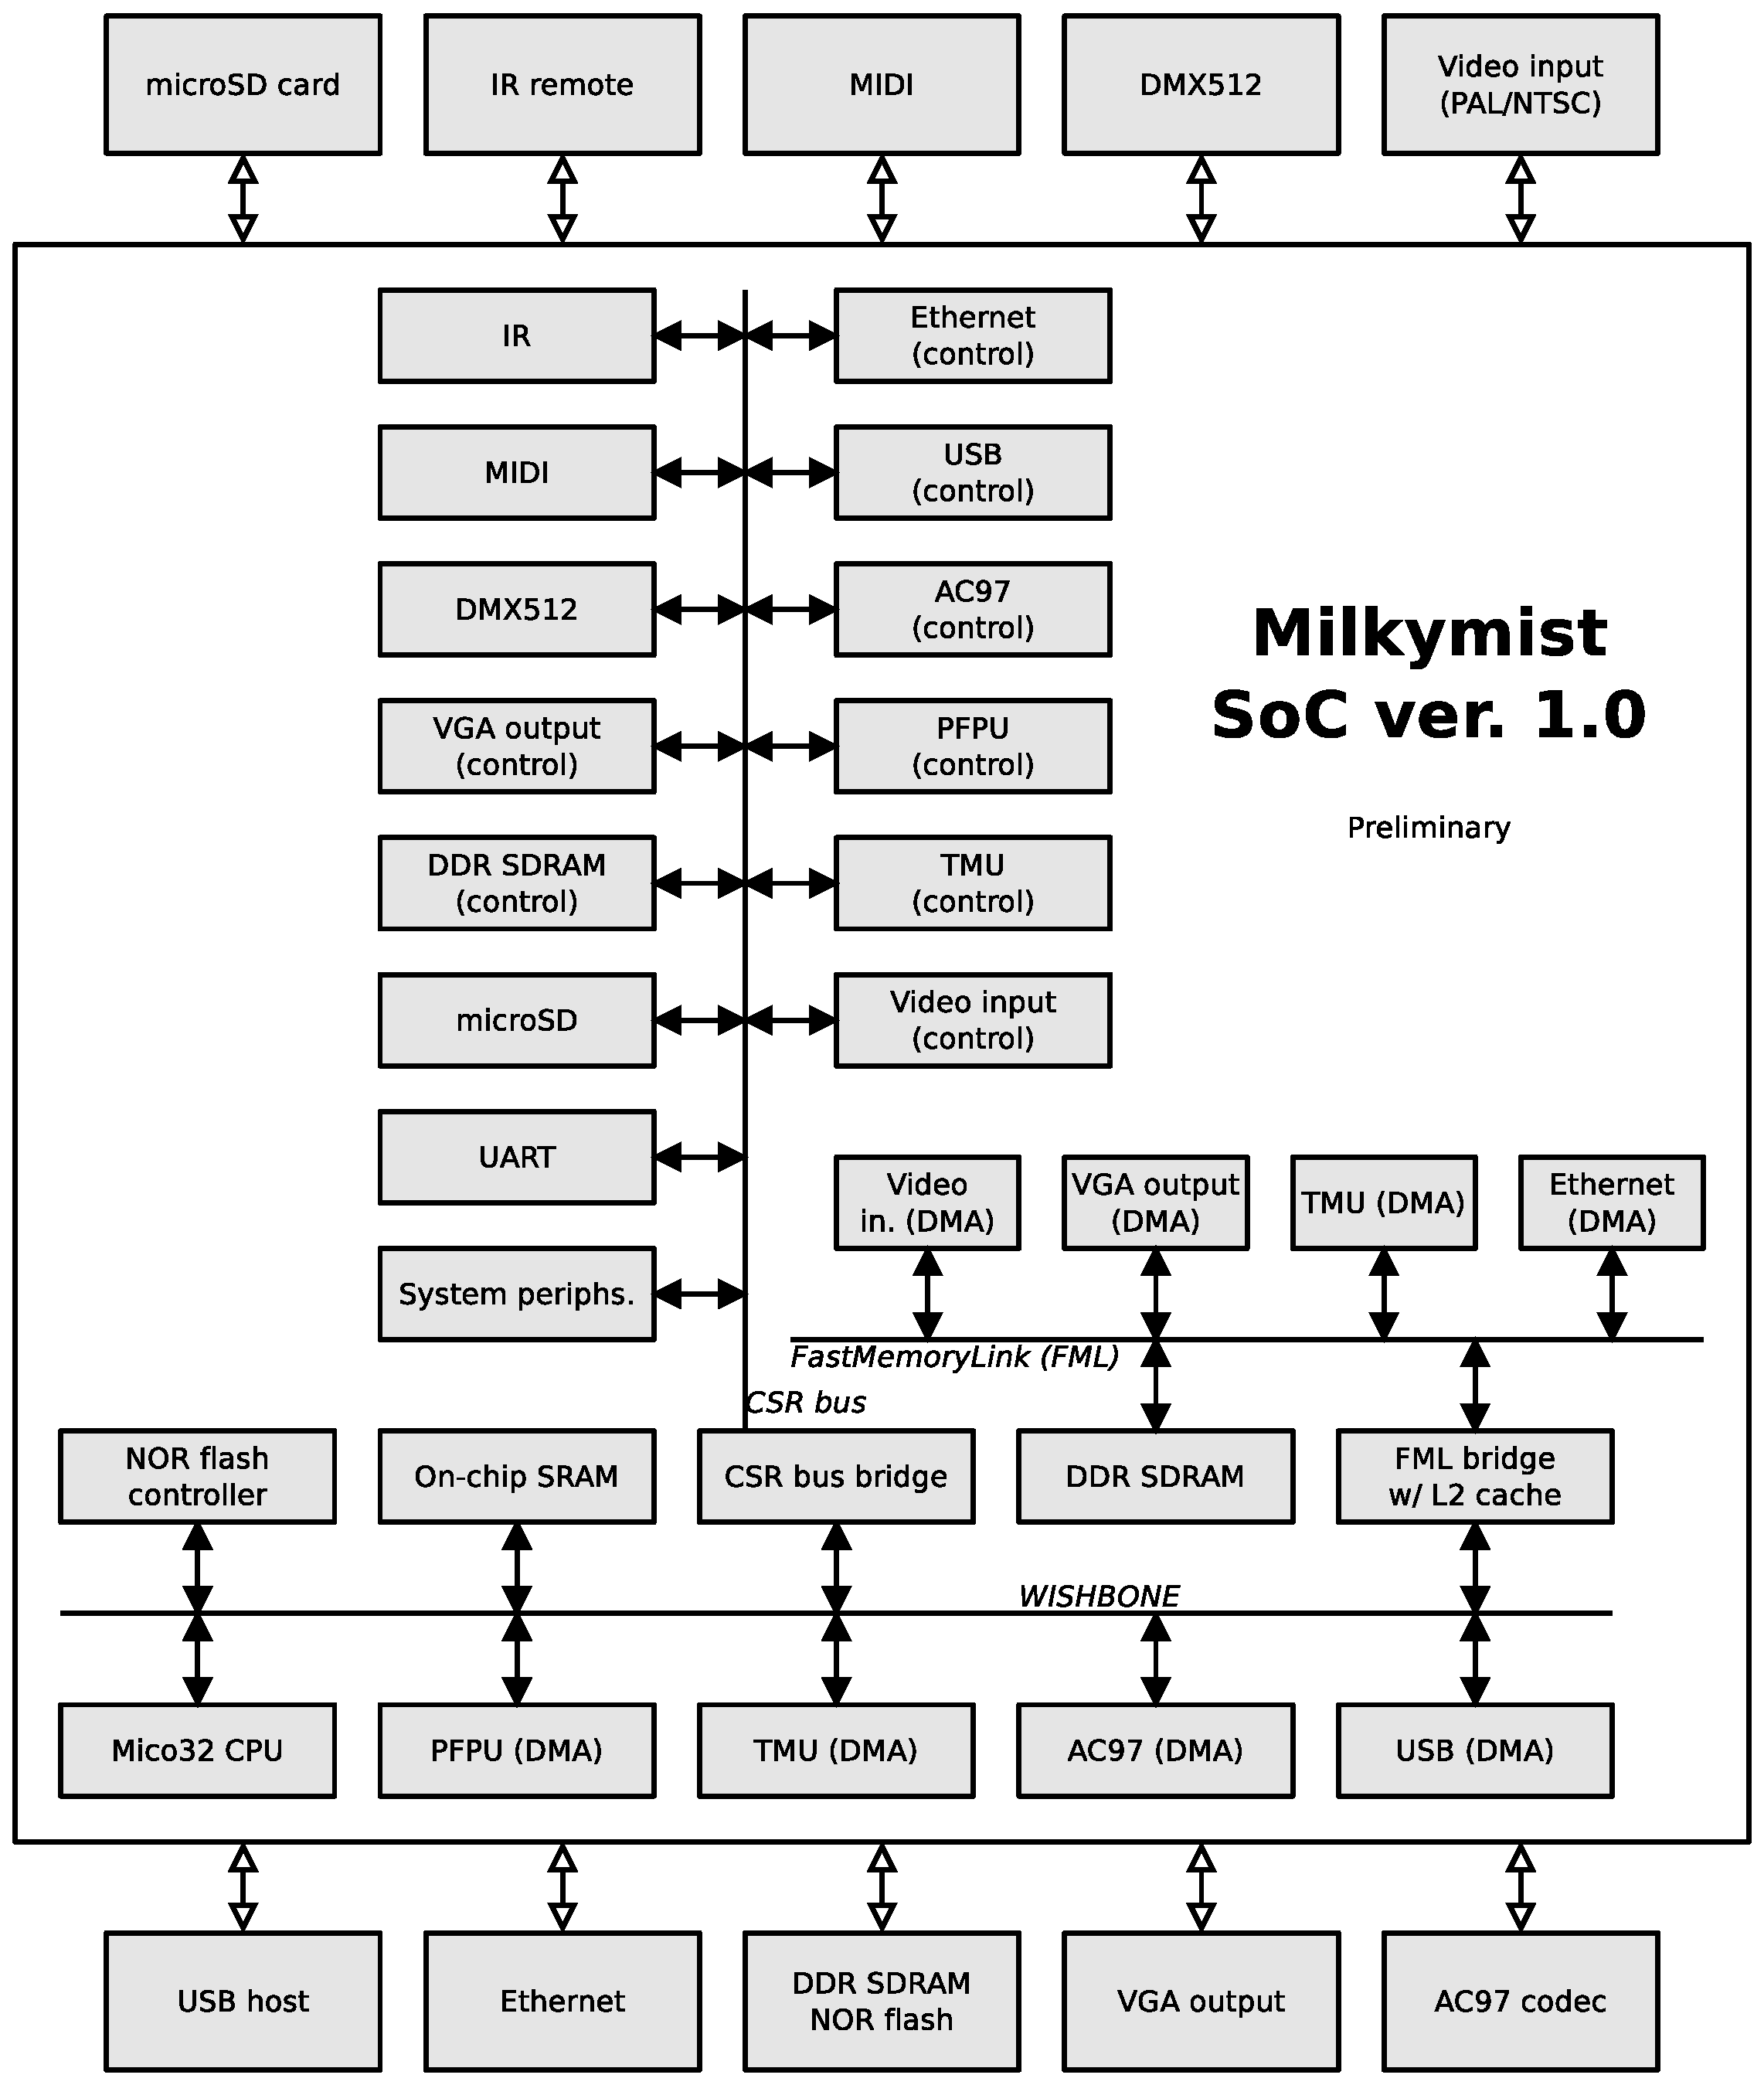
\includegraphics[height=130mm]{soc_architecture.eps}
\caption{SoC block diagram}
\label{fig:block}
\end{figure*}

\subsection{SoC interconnect}
The Milkymist system-on-chip uses three different kind of buses :
\begin{itemize}
\item WISHBONE~\cite{wishbone} as a general purpose bus around the CPU core.
\item a custom ``CSR'' bus~\cite{csr} used to access configuration and status registers of peripherals. It is simpler than WISHBONE; it does not support variable latency and the address decoding is simplified.
\item a custom ``FastMemoryLink'' (FML) bus~\cite{fml} which is pipelined and burst-oriented for efficient DRAM access.
\end{itemize}
By removing the need for logic that is only required to comply with a too general bus specification, the use of these specific buses reduce the hardware design effort and improve resource efficiency.

\subsection{Building blocks}
\subsubsection{Base system}
The base system is made up of a Mico32 CPU core~\cite{mico32}, on-chip SRAM, off-chip Flash, an UART for printing debug messages, general-purpose I/O ports, timers, and interrupt controller.

The Mico32 core can execute uClinux~\cite{micolinux}, or be programmed like a microcontroller, without operating system.

There are plans to use AEMB~\cite{aemb} instead of Mico32.

These make up a basic system that is capable of executing software and communicate with the outside world. On top of this system, special peripherals and accelerators are added.

\subsubsection{Memory interface}
The system-on-chip is equipped with a custom DDR SDRAM controller~\cite{hpdmc}, supporting a FastMemoryLink interface.

The DDR SDRAM data bus width is 32 bits and is running at 100MHz, delivering a peak (ideal) memory bandwidth of 6.4Gbps.

The memory controller is fully synchronous (the SDRAM clock is the system clock) to avoid clock domain crossing delays and reduce the overall memory latency.

It is a ``page mode'' controller, which leaves DRAM pages open after an access on the chance that the next access will be on the same page. This has been shown to be fruitful in most cases~\cite{pagemode}.

Memory latencies are further reduced by the use of pipelined transfers on the FML bus.

\subsubsection{VGA output}
The system-on-chip directly drives the H/V synchronization pins of the VGA interface and a video DAC that generates the red, green and blue analog signals.

The framebuffer is read from DRAM using the FML interface directly.

To cope with the hard realtime constraint of the video signal generation, the VGA controller contains a FIFO which hides the memory latencies.

The framebuffer uses a simple progressive scan 16bpp RGB565 schema. The controller supports multiple buffering and synchronizes the switching between the framebuffers with the vertical blanking intervals in order to prevent drawing artifacts.

\subsubsection{Texture mapping unit (TMU)}
The unit maps a texture on a surface defined by a triangle strip.

To implement MilkDrop at a good frame rate, this becomes a very computation and memory intensive process. The implementation is heavily parallel, and is directly connected to the FML bus to acheive memory bandwidth constraints~\cite{confslides}~\cite{tmu}.

\subsubsection{Programmable floating point unit (PFPU)}
The PFPU~\cite{pfpu} is a floating point coprocessor, whose primary purpose is generating vertex data when implementing MilkDrop.

It is a pipelined VLIW processor with all the scheduling done by the compiler. Loop structures are not programmable, which limits the use case to evaluating mathematical expressions.

\subsubsection{Audio I/O}
The audio controller interfaces the system-on-chip to industry-standard and cheap AC97 codecs.

\subsubsection{Memory card}
The system is equipped with a CompactFlash memory card controller, which is used to store firmware, and user media and data.

\subsubsection{Video inputs}
Two video inputs compatible with PAL and NTSC are planned to be added to the system. 

An external ADC and decoder chip like ADV7181 will be added to simplify the process.

Those video inputs enable the use of the device in live video mixing and transformation applications.

\subsubsection{Control peripherals}
The following interfaces are planned to be added to the system :
\begin{itemize}
\item DMX512 (stage lighting)
\item MIDI (electronic instruments)
\item Ethernet (OpenSoundControl for electronic instruments)
\end{itemize}

These make the device suitable for artistic installations and performances.

\section{Development system}
The system is currently working on a Xilinx ML401 development board equipped with a Virtex-4 XC4VLX25 FPGA. This board integrates most of the peripherals, except DMX512, MIDI and video inputs.

A custom PCB is in development, which will be smaller, have all the interfaces and use a cheaper Spartan-3A FPGA.

On the software side:
\begin{itemize}
\item ISE Webpack from Xilinx synthesizes the FPGA bitstream,
\item Verilog simulations are run with GPL Cver~\cite{gplcver} and Icarus Verilog~\cite{icarus},
\item GCC is used to compile the code for the SoC's CPU.
\end{itemize}

All these tools are either free (as in freedom) or available at no charge.

\section{Conclusion}
Milkymist features a powerful system-on-chip design, perfectly suited for running embedded applications targeted at video performance artists (VJs). It is also fully open-source (GNU GPL license version 3), flexible and well documented, allowing its components to be re-used in other system-on-chip designs.

\bibliography{paper_overview}{}
\bibliographystyle{plain}

\end{document}
